\documentclass[12pt]{article}

\usepackage[utf8]{inputenc}
\usepackage{latexsym,amsfonts,amssymb,amsthm,amsmath}

\setlength{\parindent}{0in}
\setlength{\oddsidemargin}{0in}
\setlength{\textwidth}{6.5in}
\setlength{\textheight}{8.8in}
\setlength{\topmargin}{0in}
\setlength{\headheight}{18pt}
\usepackage{graphicx} % Required for inserting images

\usepackage{listings}

\usepackage{xcolor}

\usepackage{booktabs}

\usepackage[toc]{appendix}

\title{Econometría 2502 - Taller 1}
\author{Rafael Marulanda, Carlos Puerto y Lorena Toro}
\date{Agosto 2025}

\begin{document}

\maketitle

\section{Experimento hipotético}

Impacto del acceso a armas de fuego en la agresividad.

\begin{itemize}
    \item Diseñe un experimento controlado ideal hipotético para estudiar si el acceso a armas de fuego incrementa la agresividad en individuos de distintas edades.

    \item ¿Cuáles serían los principales impedimentos éticos para llevar a cabo este experimento?

    \item Si solo se contara con datos observacionales de personas que han crecido en entornos con mayor acceso a armas, ¿qué variables de control podrían afectar los resultados?

    \item ¿Cómo podría abordarse este tema sin poner en riesgo la seguridad de los participantes o del público?
\end{itemize}

\subsection{Diseño del experimento}

\subsubsection{Objetivo} 

Determinar si introducir un arma de fuego en la casa aumenta actitudes agresivas o comportamiento agresivo en sus ocupantes después de dos años. 

\subsubsection{Participantes} 300 Familias que no hayan usado armas de fuego antes. 

\subsubsection{Metodología} 

\begin{enumerate}
\item Los participantes se someten a evaluaciones psicológicas para tener una línea base de agresión, impulsividad y formas de resolver conflictos. 

\item Las familias se asignan aleatoriamente a dos grupos: 
\begin{itemize}

\item Un grupo experimental en el que a la familia se le da un arma de fuego desactivada en una caja de seguridad. Reciben entrenamiento riguroso en armas de fuego. 

\item Un grupo de control en el que a la familia se le da una caja de seguridad idéntica vacía y recibe el mismo tratamiento del grupo anterior. 

\end{itemize}

\end{enumerate}

\subsubsection{Recolección y análisis de datos} 


\begin{itemize}
\item Se hacen evaluaciones de seguimiento periódicas, y se recolectan los datos. 

\item Se recolectan los reportes laborales y disciplinarios de los miembros del hogar. 

\item Los investigadores compararán los cambios en los niveles de agresión y comportamiento entre los dos grupos. 


\end{itemize}


\subsection{Impedimentos éticos}
\begin{itemize}
\item Meter un arma de fuego en una casa (aunque esté desactivada) es irresponsable. 

\item Permitir estas armas de fuego podría crear fascinación en los habitantes de la casa. 

\item No se debe tratar a los seres humanos como herramientas en un experimento con riesgos psicológicos.

\end{itemize}

\subsection{Variables de control que podrían afectar los resultados}

\begin{itemize}
\item Niveles de pobreza y desigualdad. 

\item Tasa de criminalidad del barrio. 

\item Nivel educativo de los padres.

\end{itemize}

\subsection{Alternativa al experimento}

Se podrían comparar las tasas de crímenes violentos entre países con leyes de armas muy estrictas y países con leyes laxas. 
Así se podrían identificar tendencias y correlaciones a gran escala que afectan a millones de personas.

\section{Problema de Combinatoria}
Una agencia automotriz recibe un lote de 20 automóviles nuevos, de los cuales 2 presentan defectos. Para decidir si acepta el embarque, la agencia selecciona al azar 2 automóviles y lo aprueba solo si ninguno de los vehículos escogidos tiene defectos. ¿Cuál es la probabilidad de que el embarque sea aceptado?

\begin{itemize}
    \item Número total de carros: $n = 20$
    \item Carros buenos: $18$
    \item Carros defectuosos: $2$
\end{itemize}

Se seleccionan dos carros, y se aprueba si los dos están bien.

\textbf{El problema es:} Combinatoria sin reemplazo.
\begin{itemize}
    \item Se escogen $r=2$ carros de $n=20$.
    \item El número total de combinaciones posibles es: $\binom{n}{r}=\binom{20}{2}=\frac{20!}{2!(20-2)!}=\frac{20 \times 19}{2 \times 1}=190$.
    \item El experimento es aceptado si 2 carros salen buenos. Hay 18 carros buenos.
    \item Las posibles combinaciones de carros buenos son: $\binom{18}{2}=\frac{18!}{2!(18-2)!}=\frac{18 \times 17}{2 \times 1}=153$.
    \item La probabilidad de aceptación es: $\frac{153}{190} \approx 0.805$.
    \item Realizando el producto entre 0.805 y 100 se obtiene un 80.5\%
\end{itemize}

\section{Problema de combinación}

En una empresa existen 18 individuos en su personal ¿cuántos equipos de trabajo (incluyendo el equipo vacío y el completo) sería posible constituir?

\begin{itemize}
    \item Hay $n=18$ trabajadores.
    \item ¿Cuántos son los posibles subconjuntos que podemos formar, incluyendo el conjunto vacío ($\emptyset$) y todos?
    \item Cada trabajador tiene dos posibilidades: estar en el equipo o no. Y son independientes.
    \item El total de subconjuntos es $2^{n}=2^{18}=262144$.
\end{itemize}

\section{Problema de combinación}

Existen 25 estudiantes en su salón de clases ¿de cuantas maneras se puede seleccionar dos representantes estudiantiles?\\

Este es un caso de combinación, ya que, como se pide dos representantes (es decir van a ejercer las mismas funciones) el orden de selección no importa, luego se aplica la formula: nCr, donde n=25 (el total de estudiantes) y r=2 (el numero de plazas para representación.)
Aplicando la formula $nCr= \frac{n!}{r!(n-r)!}$\\

Ahora, reemplanzado con los valores la formula se tiene que $25C2= \frac{25!}{2!(25-2)!}=300$ formas de selecciónar dos representantes.

\section{Problema de combinación}

La junta directiva de una empresa se encuentra conformada por 10 mujeres y 6 hombres ¿de cuantas maneras puede conformarse un comité de 4 personas tal que se cumplan las siguientes condiciones?

\begin{itemize}
    \item Todos los cuatro sean hombres.
    \item Todos los cuatro sean mujeres.
    \item Dos sean hombres y dos mujeres.
    \item Por lo menos uno sea hombre.
\end{itemize}

Este es un caso de combinación dado que para la selección del comité no se exige un orden. No obstante, dadas las condiciones anteriores se hace necesario dividr el problema en partes generando nuevos comotes a partir de dichas condciones. Como la primera condición exige que el comité de 4 sea compuesto por solo hombres, al conjunto total n=16 se debe restar el subconjunto de mujeres, luego quedara $n=(16-10)=6$.\\

De este subconjunto formado por hombres se seleccionará el primer comité, así, se tiene que n=6 y r=4, aplicando la formula de combinación nCr se tiene $6n2=\frac{6!}{2!(4-2)!}$ dando como resultado 15 maneras para realizar la selección.\\

La segunda condición establece que el comité este formado por solo mujeres, aplicando $n=(16-6)=10$ se obtiene que en este caso $n=10$ que es el subconjunto formado por mujeres de las cuales se seleccionara el comité formado por $r=4$. Aplicando la formula nCr se tiene $\frac{10!}{4!(6)!} = 210$ formas de seleccionar el comité entre mujeres.\\

Ahora bien, la tercera condición establece que el comité debe estar compuesto por dos hombres y dos mujeres. En este caso se aplica la formula anterior pero haciendo r=2 para cada subconjunto de hombres y mujeres, luego el producto de cada combinación es el numero de formas que se puede seleccionar el comité.\\

(1)	Para el caso de los hombres $n=6$ y $r=2$, se aplica nCr, obteniendo  15 maneras de formar el comité.\\
(2)	Para el caso de las mujeres $n=10$ y $r=2$ se aplica nCr, obteniendo 45 maneras de formar el comité.\\
Finalmente se realiza el producto entre (1) y (2) obteniendo 675 formas de organizar el comité teniendo dos hombres y dos mujeres.\\
\\\\La última condición establece que por lo menos un miebro del comité sea hombre. Para este caso se debe proceder de la siguiente manera: (1) Se debe realizar la combinación del total del conjunto $n=16$ con el número de plazas $r=4$ dando por resultado $16n4=1820$. (2) Se procede con la combinación del conjunto de mujeres $n=10$ y $r=4$ dando por resultado $10c4=210$.
\\\\Ahora se realiza la diferencia entre (1) y (2) dando por resultado 1610 formas de organizar los comites teninedo al menos un hombre.\\
    
\section{Problema de permutación}

En un laboratorio clínico, se realizan pruebas para diagnosticar 3 tipos de enfermedades: viral, bacteriana y parasitaria. Para cada paciente, el médico puede ordenar 2 tipos de pruebas diferentes (de un catálogo de 5 pruebas). ¿De cuántas maneras distintas puede el médico ordenar las pruebas si el orden en que se realizan importa?\\

Este es un caso de permutación en el cual, si bien se dice que se pueden diagnosticar tres tipos de enfermedades, tan solo es posible mandar 2 pruebas del total de 5. De lo cual se sigue que, aunque se puedan diagnosticar tres tipos distintos tan solo se puede tener registro de máximo 2 (dado el número de pruebas que se pueden mandar), luego el total de pruebas es $n=5$ y el número de elementos a ser tomados es $r=2$.\\

Como el orden de aplicación importa (debido a que no es lo mismo ser diagnosticado con una enfermedad bacteriana, parasitaria o viral) se debe aplicar la fórmula de permutación quedando así nPr. Reemplazando con los valores queda $nPr=\frac{5!}{(5-2)!}= 20$ maneras bajo las cuales puede el doctor ordenar las pruebas.\\

\section{Problema de probabilidad}

En un hospital, el 20\% de los pacientes en urgencias tienen fiebre, el 35\% tienen tos y el 10\% tienen ambas. Si se selecciona un paciente al azar, ¿cuál es la probabilidad de que tenga fiebre o tos?\\

Este es un caso de probabilidad de la intersección, para resolverlo se debe proceder armando la intersección de dos conjuntos. El conjunto de los pacientes con fiebre que es del 20\%, el conjunto de los que tienen tos es del 35\% y finalmente, la intersección de estos conjuntos se compone por el 10\% que tienen tanto tos como fiebre. Para resolver este problema recurriremos a la formula de probabilidad de Laplace para unión de conjuntos.\\

Asumiendo que la suma total de pacientes es del 100\% se tiene que la probabilidad de ser un paciente con fiebre es igual a $P(A)=\frac{20}{100}=0.20.$ La probabilidad de ser paciente con tos es igual a $P(B)=\frac{35}{100}=0.35$. Ahora, se quiere sacar la probabilidad de que el suceso A y el suceso B ocurran en simultaneo, con ello se debe obtener $P(A\cap B)$ Sin embargo, para obtener la probabilidad de la intersección, primero debe obtenerse la probabilidad de la unión de los conjuntos, es decir $P(A\cup B)=\frac{10}{100}=0.10$.\\

Con estos datos se aplica la formula que relaciona la probabilidad de la unión de la intersección, ésta dice que: $P(A\cup  B) = P(A) + P(B) - P(A\cap  B)$ Reemplazando los valores se tiene:
        \\\\$0.10 = 0.20 + 0.35 - P(A\cap  B)$ 
\\\\$P(A\cap  B)=0.20 + 0.35 - 0.10$ 
\\\\$P(A\cap  B)= 0.45$ es la probabilidad de tener un paciente con tos y fiebre, multiplicando por 100 da como resultado 45\%.

\section{Problema de combinación de equipos}


Un quirófano debe conformar un equipo de 5 médicos a partir de 8 cirujanos y 6 anestesiólogos, garantizando que haya al menos 2 cirujanos. ¿Cuántas maneras distintas hay de formar este equipo?
\\\\Para este ejercicio se debe considerar primero el número total de casos bajo los cuales se pueden combinar los equipos cumpliendo la condición de mantener al menos 2 cirujanos dentro del equipo final. De forma que el primer caso de combinación posible sería de (1) 8C2 y (2) 6C3 dando por resultado 28 y 20, realizando el producto entre (1) y (2) se obtiene 560.
\\\\Sin embargo, esto seria en el caso de que se tuviera el valor fijo de 2 cirujanos, mas como la condición inicial indica “al menos 2” luego, se tiene que repetir esta operación con los otros posibles casos y luego realizar la adición de cada caso, así las siguientes formaciones serían [8C3,6C2], [8C4,6C1] y [8C5,6C0]. Realizando las operaciones se obtiene [840], [420] y [56].
\\\\Ahora, sumando los 4 escenarios se obtienen 1876 formas de organizar los equipos de médicos cumpliendo la condición de mantener al menos 2 cirujanos.



\section{Correlación en Stata}

Usando STATA y el generador de números aleatorios calcule para n=500
$z_i~n(0,1)$

\begin{itemize}
    \item Grafique el histograma de frecuencias de $z_i$ comente sobre sus resultados.

    \begin{figure}[h]
        \centering
        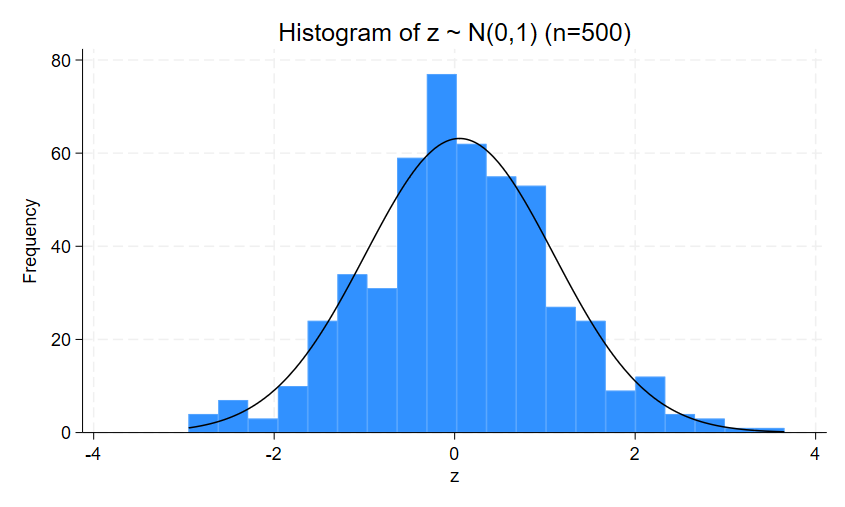
\includegraphics[width=0.75\linewidth]{Figures/hist_z.png}
        \caption{Histograma de frecuencias de $z_i$}
        \label{fig:Hist_z}
    \end{figure}

   
Este primer histograma nos indica que los datos generados se comportan como una distribución normal estándar: simétrica, centrada en 0 y con la mayor parte de datos cercanos a la media.

    \item Genere la variable $y_i=5+z_i$. Grafique el histograma de frecuencias de $y_i$ y comente sus resultados.

    \begin{figure}[h!]
        \centering
        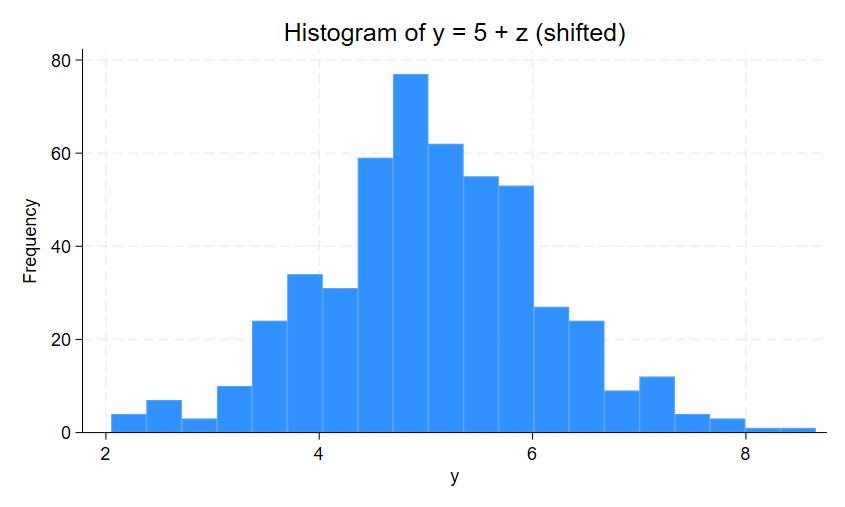
\includegraphics[width=0.75\linewidth]{Figures/hist_y.png}
        \caption{Histograma de frecuencias de $y_i$}
        \label{fig:Hist_y}
    \end{figure}

    Una distribución normal simétrica, centrada en cero es dada por z.
La distribución z se desplaza 5 unidades a la derecha, sin perder su forma para construir


$y_i=5+z_i$

Aquí solo hay desplazamiento. La dispersión es la misma, los extremos siguieron guardando la misma distancia del centro. Es la misma campana, pero desplazada.

    \item Genere la variable $w_i=5+3z_i$. Grafique el histograma de frecuencias de $w_i$ y comente sus resultados.

    \begin{figure}[h!]
        \centering
        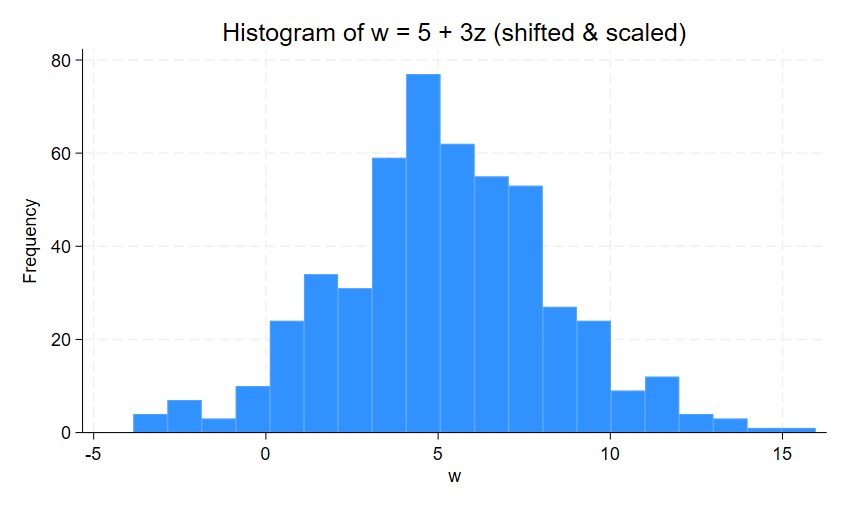
\includegraphics[width=0.75\linewidth]{Figures/hist_w.png}
        \caption{Histograma de frecuencias de $w_i$}
        \label{fig:Hist_w}
    \end{figure}

    En este último histograma, la distribución normal estándar, se ha modificado de tal forma que la media se desplaza a 5 unidades y la dispersión se ha triplicado, dando por resultado que la campana conserva su forma  pero se ha ensanchado y aplanado. La mayor parte de los datos se ubican entre un rango de 2 a 8, con una desviación estandar, casi todos entre un rango de –1 a 11. En otras palabras, al sumar la constante esta mueve la curva, mientras que multiplicar por 3 la ensancha, obteniendo que el rango se amplia con valores probables sin alterar distribución normal.

    \item Calcule la correlación en parejas entre $z_i$, $y_i$ y $w_i$ usando STATA. Luego calcule a mano la correlación entre las mismas variables. Muestre y comente sus resultados.

    \begin{table}[h!]
    \centering
    \caption{Mariz de correlaciones dadas por Stata}
    \begin{tabular}{lccc}
    \hline
                & $z$     & $y$     & $w$     \\
    \hline
    $z$         & 1.0000  &         &         \\
    $y$         & 1.0000  & 1.0000  &         \\
    $w$         & 1.0000  & 1.0000  & 1.0000  \\
    \hline
    \end{tabular}
    \end{table}   
    
\end{itemize}

\section{Distribución $\chi^2$ en Stata}

Usando STATA y el generador de números aleatorios calcule las siguientes variables para n=250: 

$x_i \sim N(0,1)$ y $y_i \sim \chi_5^2$

\begin{itemize}
    \item Estime usando el comando sum el valor esperado y la varianza de las dos variables aleatorias. Muestre sus resultados. Además, calcule el histograma y la función kernel de cada una de las variables. Muestre sus resultados.

    Con \texttt{sum} en Stata se obtuvieron los siguientes estadísticos muestrales (\(n=250\)):

    \begin{table}[h!]
    \centering
    \caption{Media y varianza muestral}
    \begin{tabular}{lrrrrr}
    \hline
    Variable & Obs & Media & Desv.\ est.\ & Mín & Máx \\
    \hline
    $x$ & 250 & $-0.0251$ & $0.9892$ & $-2.5481$ & $2.8004$ \\
    $y$ & 250 & $5.2475$  & $3.5384$ & $0.3989$  & $18.4825$ \\
    \hline
    \end{tabular}
    \end{table}
    
    \vspace{0.5em}
    A continuación se presentan los histogramas junto con la densidad kernel (KDE) estimada para cada variable:
    
    \begin{figure}[h!]
    \centering
    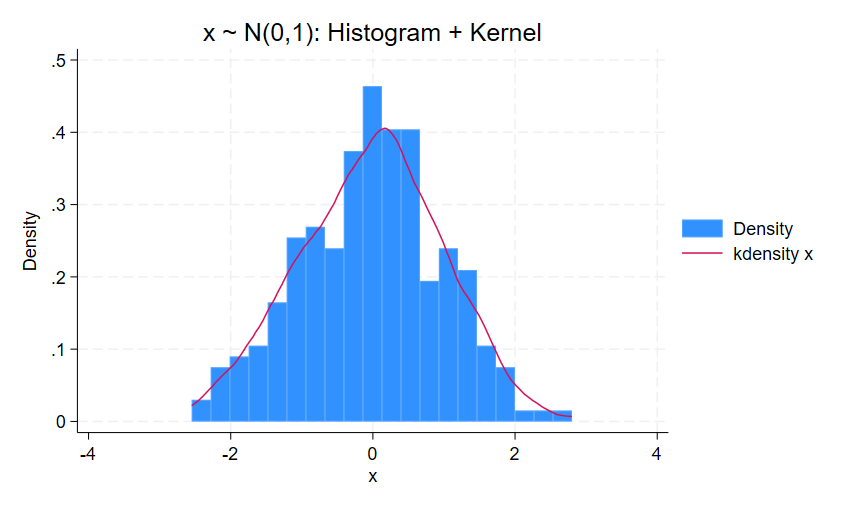
\includegraphics[width=.48\textwidth]{Figures/0110_hist_x.png}\hfill
    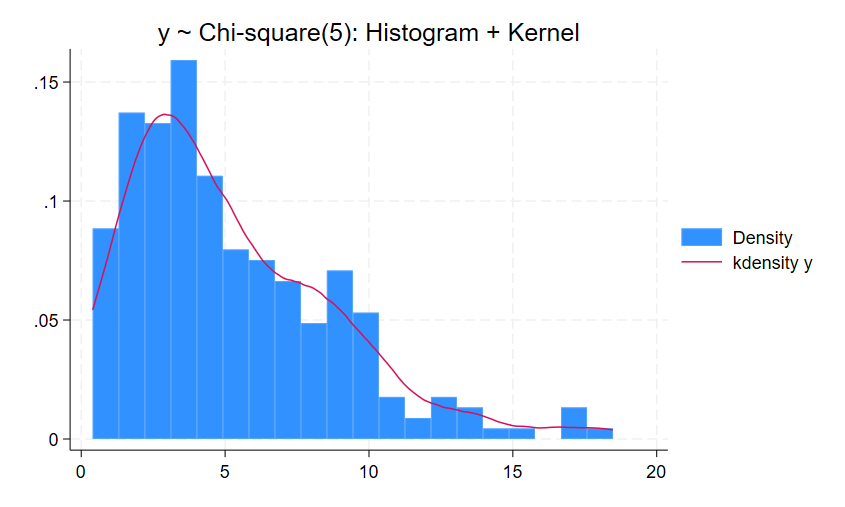
\includegraphics[width=.48\textwidth]{Figures/0110_hist_y.png}
    \caption{Histogramas y densidad kernel para $x$ (izquierda) y $y$ (derecha).}
    \end{figure}

    \item Conociendo que las dos variables se distribuyen normal y $\chi^2$ respectivamente, responda ¿Cuál es el valor esperado de una normal estándar? ¿su varianza? ¿Cuál es el valor esperado de una $\chi^2$? ¿su varianza?\\

    Si \(X \sim \mathcal{N}(0,1)\) (normal estándar), entonces
    \[
    \mathbb{E}[X]=0, 
    \qquad 
    \operatorname{Var}(X)=1.
    \]
    
    Si \(Y \sim \chi^{2}_{k}\) (chi–cuadrado con \(k\) grados de libertad), entonces
    \[
    \mathbb{E}[Y]=k, 
    \qquad 
    \operatorname{Var}(Y)=2k.
    \]
    
    \noindent para \(k=5\),
    \[
    \mathbb{E}[Y]=5, 
    \qquad 
    \operatorname{Var}(Y)=10.
    \]

    \item 	Genere las siguientes variables $W_i=ax_i, Z_i=a+x_i$. En donde $a$ equivale a la suma de los dos últimos dígitos de los números de identificación de los integrantes del grupo. Calcule la media y la varianza de estas nuevas variables aleatorias. Comente a la luz de las propiedades del valor esperado y la varianza sus resultados.\\

    Sea $X\sim\mathcal N(0,1)$ y definamos el parámetro
    \[
    a = 95+86+41 = 222.
    \]
    A partir de $X$ se construyen las variables
    \[
    W_i = aX_i, 
    \qquad 
    Z_i = a+X_i.
    \]
    
    \paragraph{Momentos teóricos por propiedades.}
    \[
    \mathbb E[W] = a\,\mathbb E[X] = 0, 
    \qquad 
    \mathrm{Var}(W) = a^2\,\mathrm{Var}(X) = a^2 = 222^2 = 49{,}284.
    \]
    \[
    \mathbb E[Z] = a + \mathbb E[X] = a = 222, 
    \qquad 
    \mathrm{Var}(Z) = \mathrm{Var}(X) = 1.
    \]
    
    La esperanza es lineal y la varianza permanece constante a los desplazamientos: 
    sumar $a$ no cambia la varianza, mientras que multiplicar por $a$ multiplica la varianza por $a^2$. 
    Por ello, $W$ conserva la media de $X$ (cero) pero con varianza muy grande ($a^2$), 
    mientras que $Z$ traslada su media a $a$ y mantiene la misma varianza de $X$.
    
    \paragraph{Resumen estadístico para $n=250$.}
    
    \begin{table}[h!]
    \centering
    \caption{Momentos teóricos y muestrales de $W$ y $Z$}
    \begin{tabular}{lcccc}
    \toprule
    Variable & $\mathbb E[]$ Teórico & Media Muestral & $\mathrm{Var}()$ Teórica & Varianza Muestral \\
    \midrule
    $W = aX$ & $0$   & $-5.57$   & $49{,}284$ & $48{,}202$ \\
    $Z = a+X$ & $222$ & $221.97$  & $1$        & $0.98$ \\
    \bottomrule
    \end{tabular}
    \end{table}
    
    \paragraph{Comparación.}
    Los resultados empíricos concuerdan con los valores teóricos: la media de $W$ fluctúa en torno a $0$ y su varianza es del orden de $a^2$, mientras que la media de $Z$ es cercana a $222$ y su varianza próxima a $1$. Las pequeñas discrepancias son atribuibles al error muestral debido al tamaño finito de la muestra.
    
\end{itemize}

\section{Distribución t-student en Stata}

Usando STATA corra el siguiente código:

\lstinputlisting[label=lst:inpu0111]{Code/input_hwrk-0111.do}

\begin{itemize}

    \item Calcule el valor de la función de densidad de la distribución: normal y t-student. Para la t utilice: 1,5 y 100 grados de libertad. Luego, grafique sus resultados. Para ello puede usar el comando twoway. Por ejemplo, de la forma: twoway (line n normal). Compare sus resultados en términos de los momentos de las distribuciones.

    Sea \(x \in \mathbb{R}\). Las funciones de densidad utilizadas son:
    \[
    f_{\mathcal N(0,1)}(x)=\frac{1}{\sqrt{2\pi}}\exp\!\left(-\frac{x^{2}}{2}\right),\qquad
    f_{t_\nu}(x)=\frac{\Gamma\!\left(\frac{\nu+1}{2}\right)}{\sqrt{\nu\pi}\,\Gamma\!\left(\frac{\nu}{2}\right)}
    \left(1+\frac{x^{2}}{\nu}\right)^{-\frac{\nu+1}{2}},
    \]
    donde \(t_\nu\) es la t--Student con \(\nu\) grados de libertad.
    
    Con Stata se generó una malla \(i = (\_n-50)/25\) para \(n=1,\dots,100\) y se evaluaron \(f_{\mathcal N(0,1)}(i)\), \(f_{t_1}(i)\), \(f_{t_5}(i)\) y \(f_{t_{100}}(i)\). El gráfico superpone las cuatro densidades.
    
    \begin{figure}[h!]
    \centering
    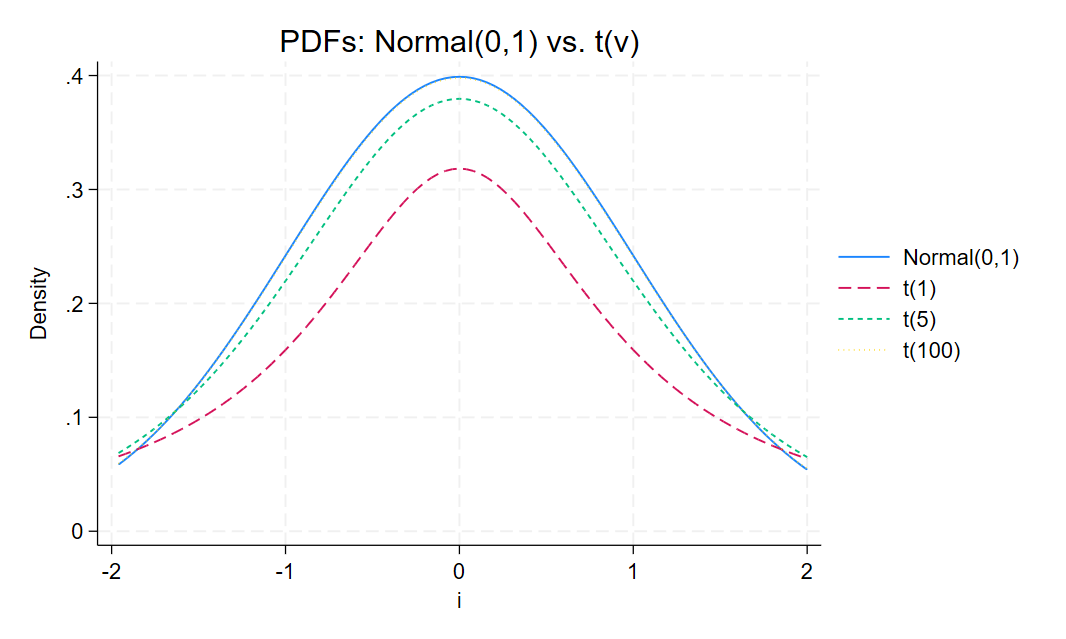
\includegraphics[width=.8\textwidth]{Figures/0111-pdfs.png}% reemplace por el nombre de su archivo exportado
    \caption{Funciones de densidad: \(\mathcal N(0,1)\) y \(t_\nu\) con \(\nu=1,5,100\).}
    \label{fig:pdfs_normal_t}
    \end{figure}
    
    \paragraph{Momentos teóricos y comparación.}
    Para la normal estándar se tiene \(\mathbb{E}[X]=0\) y \(\mathrm{Var}(X)=1\).
    Para \(t_\nu\), \(\mathbb{E}[T]=0\) si \(\nu>1\) y \(\mathrm{Var}(T)=\nu/(\nu-2)\) si \(\nu>2\);
    Concretamente, en los tres casos solicitados:
    
    \begin{table}[h!]
    \centering
    \caption{Momentos teóricos}
    \begin{tabular}{lcc}
    \hline
    Distribución & \(\mathbb{E}[\cdot]\) & \(\mathrm{Var}(\cdot)\) \\
    \hline
    \(\mathcal N(0,1)\) & \(0\) & \(1\) \\
    \(t_{1}\) & \text{no definida} & \text{no definida} \\
    \(t_{5}\) & \(0\) & \(5/(5-2)=1.6667\) \\
    \(t_{100}\) & \(0\) & \(100/(100-2)=1.0204\) \\
    \hline
    \end{tabular}
    \end{table}
    
    \noindent En la Figura~\ref{fig:pdfs_normal_t} se observa que, a medida que \(\nu\) aumenta,
    la \(t_\nu\) se aproxima a \(\mathcal N(0,1)\): la \(t(1)\) presenta el pico más bajo; la \(t(5)\) es más próxima pero aún con varianza mayor; y la \(t(100)\) prácticamente coincide con la normal.

    \item Utilizando el generador de números aleatorios de STATA y 10.000 observaciones, genere números aleatorios de las anteriores distribuciones, estime su media, varianza, asimetría y curtosis. Compare sus resultados. Grafique los histogramas de cada una de las variables.

    Se generaron \(n=10{,}000\) observaciones usando el generador aleatorio de \texttt{Stata} para
    \(\mathcal N(0,1)\) y \(t_\nu\) con \(\nu\in\{1,5,100\}\).
    Se estimaron media, varianza, asimetría y curtosis.
    
    \begin{table}[h!]
    \centering
    \caption{Momentos muestrales y teóricos}
    \label{tab:moments}
    \begin{tabular}{lrrrrrrrr}
    \toprule
    & \multicolumn{4}{c}{Muestral} & \multicolumn{4}{c}{Teórico} \\
    \cmidrule(lr){2-5}\cmidrule(lr){6-9}
    Distribución & Media & Var. & Asim. & Curt. & \(\mathbb E[\cdot]\) & \(\mathrm{Var}(\cdot)\) & Asim. & Curt. \\
    \midrule
    \(\mathcal N(0,1)\) &  0.0123 & 0.9937 &  0.0157 & 3.0464 & 0 & 1.0000 & 0 & 3.0000 \\
    \(t(1)\)            &  1.9715 & 37737.112 & 82.8366 & 7695.1467 & \multicolumn{4}{c}{no definidos} \\
    \(t(5)\)            & -0.0169 & 1.6404 & -0.0962 & 6.2563 & 0 & 1.6667 & 0 & 9.0000 \\
    \(t(100)\)          & -0.0106 & 1.0252 &  0.0184 & 2.9971 & 0 & 1.0204 & 0 & 3.0625 \\
    \bottomrule
    \end{tabular}
    \end{table}
    
    \begin{table}[h!]
    \centering
    \caption{Desviaciones muestral $-$ teórico}
    \label{tab:deviations}
    \begin{tabular}{lrrrr}
    \toprule
    Distribución & \(\Delta\)Media & \(\Delta\)Var. & \(\Delta\)Asim. & \(\Delta\)Curt. \\
    \midrule
    \(\mathcal N(0,1)\) &  0.0123 & -0.0063 &  0.0157 &  0.0464 \\
    \(t(1)\)            &    \multicolumn{4}{c}{n/a} \\
    \(t(5)\)            & -0.0169 & -0.0262 & -0.0962 & -2.7437 \\
    \(t(100)\)          & -0.0106 &  0.0048 &  0.0184 & -0.0654 \\
    \bottomrule
    \end{tabular}
    \end{table}
    

    Para \(t(1)\) los momentos teóricos no existen; la muestra produce valores extremos y una curtosis muy alta. Con \(\nu=5\) la \(t\) tiene colas pesadas (curtosis \(>3\))
    y varianza mayor que la normal. Con \(\nu=100\), \(t(100)\) se aproxima mucho más a \(\mathcal N(0,1)\).
    
    \begin{figure}[h!]
    \centering
    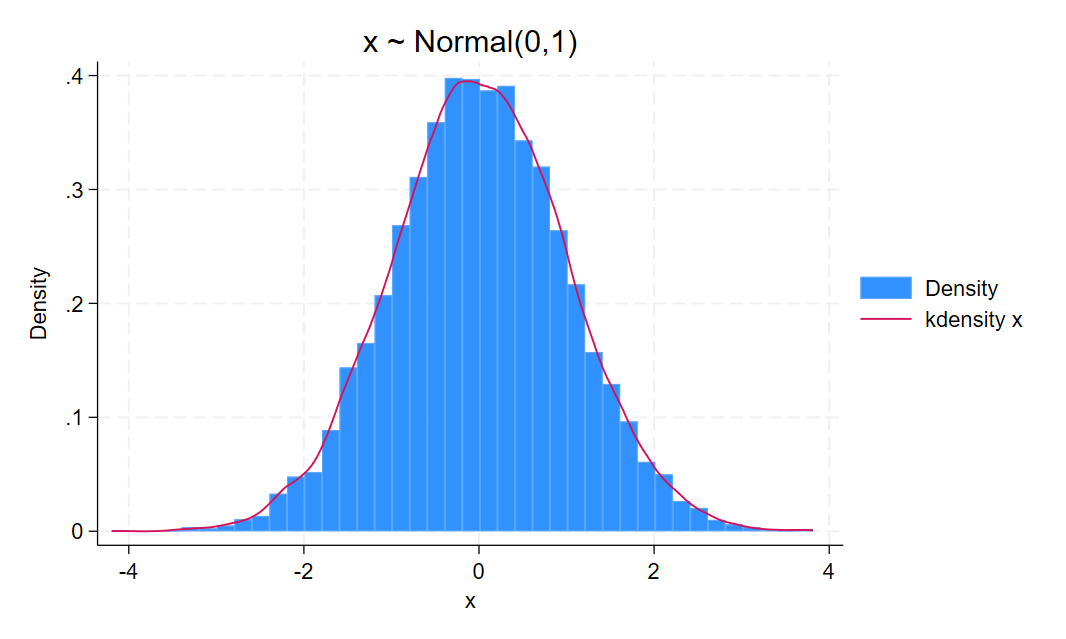
\includegraphics[width=.48\textwidth]{Figures/0111-N001.png}\hfill
    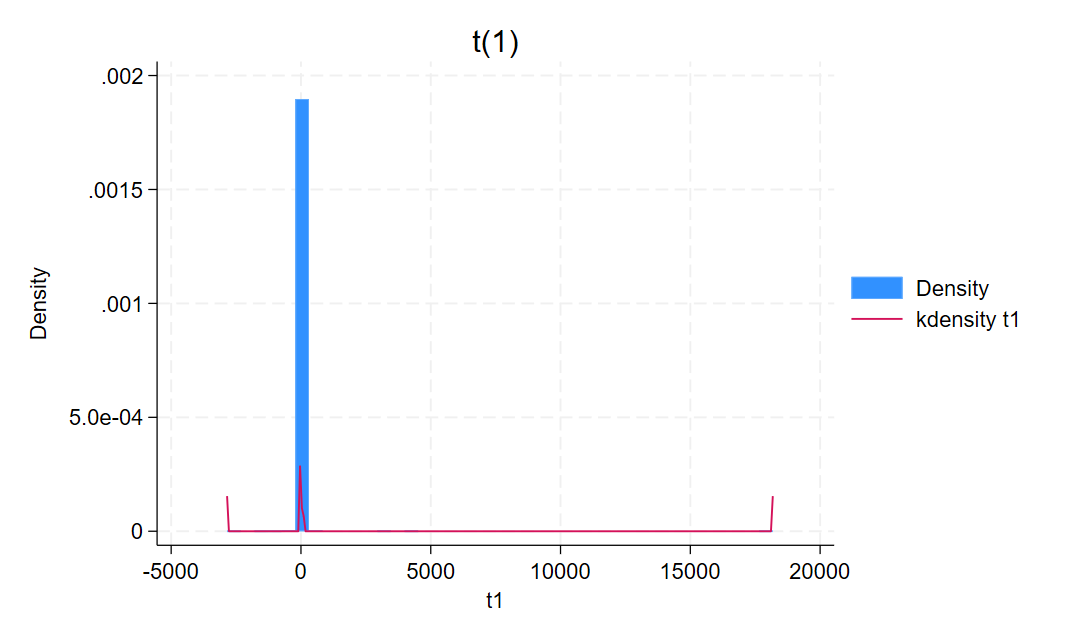
\includegraphics[width=.48\textwidth]{Figures/0111-t001.png}\\[0.4em]
    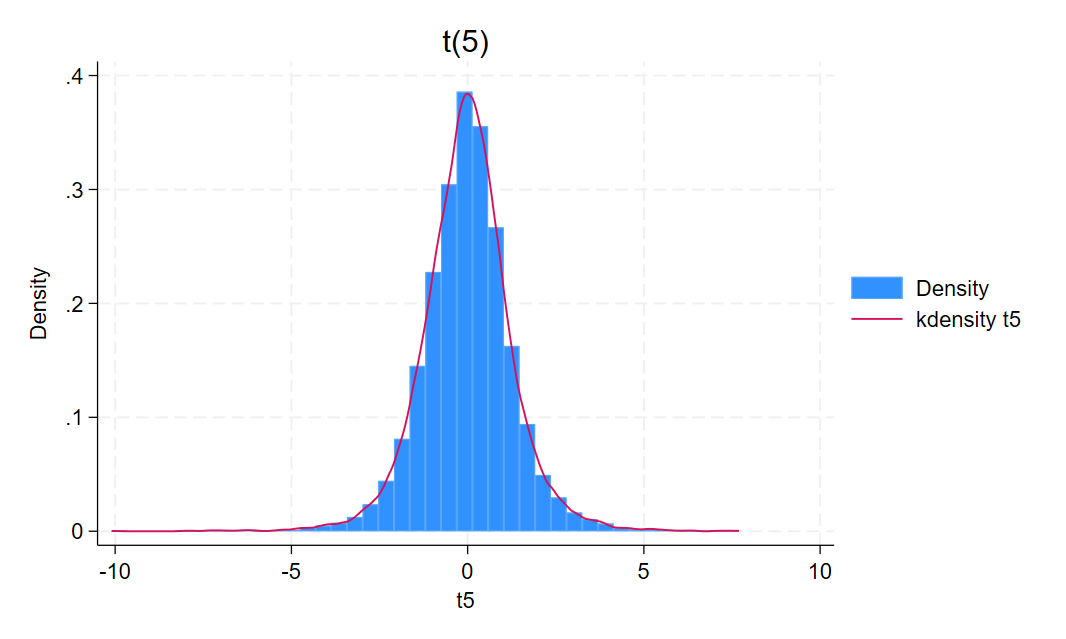
\includegraphics[width=.48\textwidth]{Figures/0111-t005.png}\hfill
    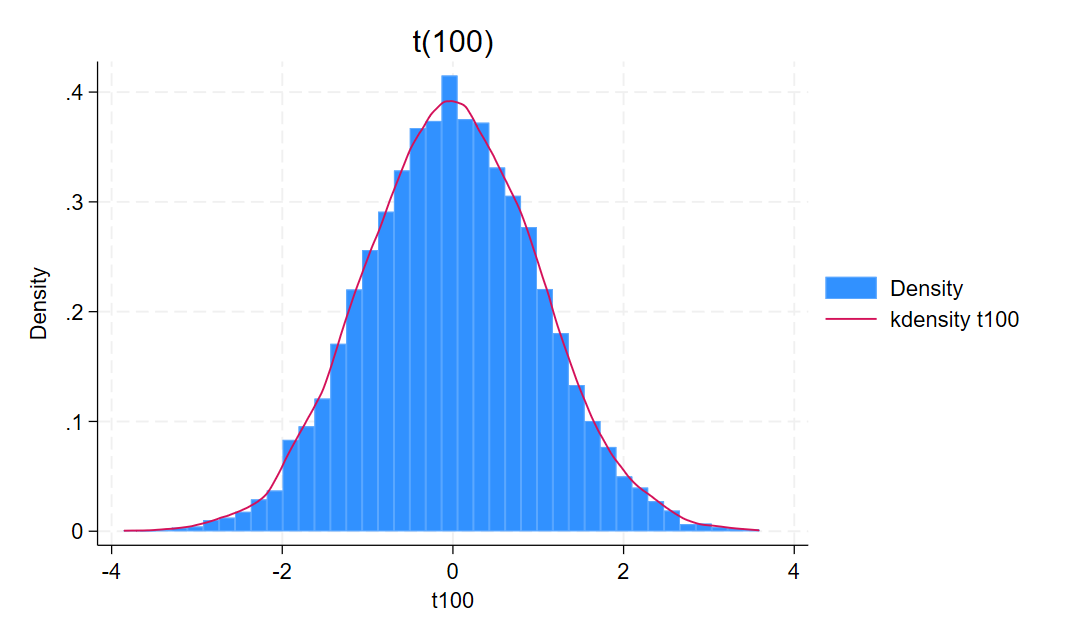
\includegraphics[width=.48\textwidth]{Figures/0111-t100.png}
    \caption{Histogramas y KDE para \(\mathcal N(0,1)\), \(t(1)\), \(t(5)\) y \(t(100)\).}
    \label{fig:hists}
    \end{figure}

    
\end{itemize}

% --- Appendix ---
\appendix
\clearpage
\section*{\centering \Huge Anexos}

\section{Código de Correlación en stata}

\lstinputlisting[label=lst:hwrk0109]{Code/ecnm-2502-hwrk-0109.do}

\section{Código de distribución $\chi^2$ en Stata}

\lstinputlisting[label=lst:hwrk0110]{Code/ecnm-2502-hwrk-0110.do}

\section{Código de distribución t-student en Stata}

\lstinputlisting[label=lst:hwrk0111]{Code/ecnm-2502-hwrk-0111.do}



\end{document}
